\chapter{基于卷积神经网络的交通标志识别}
\label{cha:seg}

\section{引言}
\label{sec:seg:introduction}

交通标志识别是无人驾驶汽车(Unmanned Ground Vehicle,UGV)和高级辅助驾驶(Advanced Driver Assistance Systems,ADAS)技术的一个重要组成部分。在驾驶行为中,驾驶员的大部分精力主要集中在结构化的道路结构和前方车辆,很容易忽视路旁小尺寸的交通标志。智能的交通标志检测可以有效地避免不必要的违章甚至交通事故。传统的计算机视觉算法曾被广泛地应用于交通标志识别任务中~\cite{le2010real},近年来卷积神经网络模型和算法的改进与完善,使得卷积神经网络在物体识别任务上取得了重大的突破。得益于计算机计算能力的提高,尤其是GPU并行计算能力的提升,使我们可以采用卷积神经网络方法去解决交通标志识别的问题。

交通标志识别并不是一个很简单任务,交通标志图像具有不同的视角、遮挡、模糊程度和尺寸变化。真实世界的环境因素也会对拍摄到的交通标志产生影响,在不同的车速、光照和天气条件下,采集到的图像会有很大的区别。此外,交通标志牌的褪色和磨损,不同时期布置的交通标志牌之间的差异等因素,都会给识别任务带来极大的困难与挑战。本章的实验对象为德国交通标志数据集(German Traffic Sign Recognition Benchmark,GTSRB)~\cite{stallkamp2012man},此数据集中的图片如图~\ref{fig:tsr_data}所示。图~\ref{fig:tsr_data}(a)列举了一些不同种类的训练交通标志样本,图~\ref{fig:tsr_data}(b)是部分不同环境因素下测试交通标志样本。德国的交通标志与大部分欧洲国家、印度和中国等国家的交通标志非常相似,是一个用于研究交通标志识别很好的公开数据集。

\begin{figure*}[t]
\centering
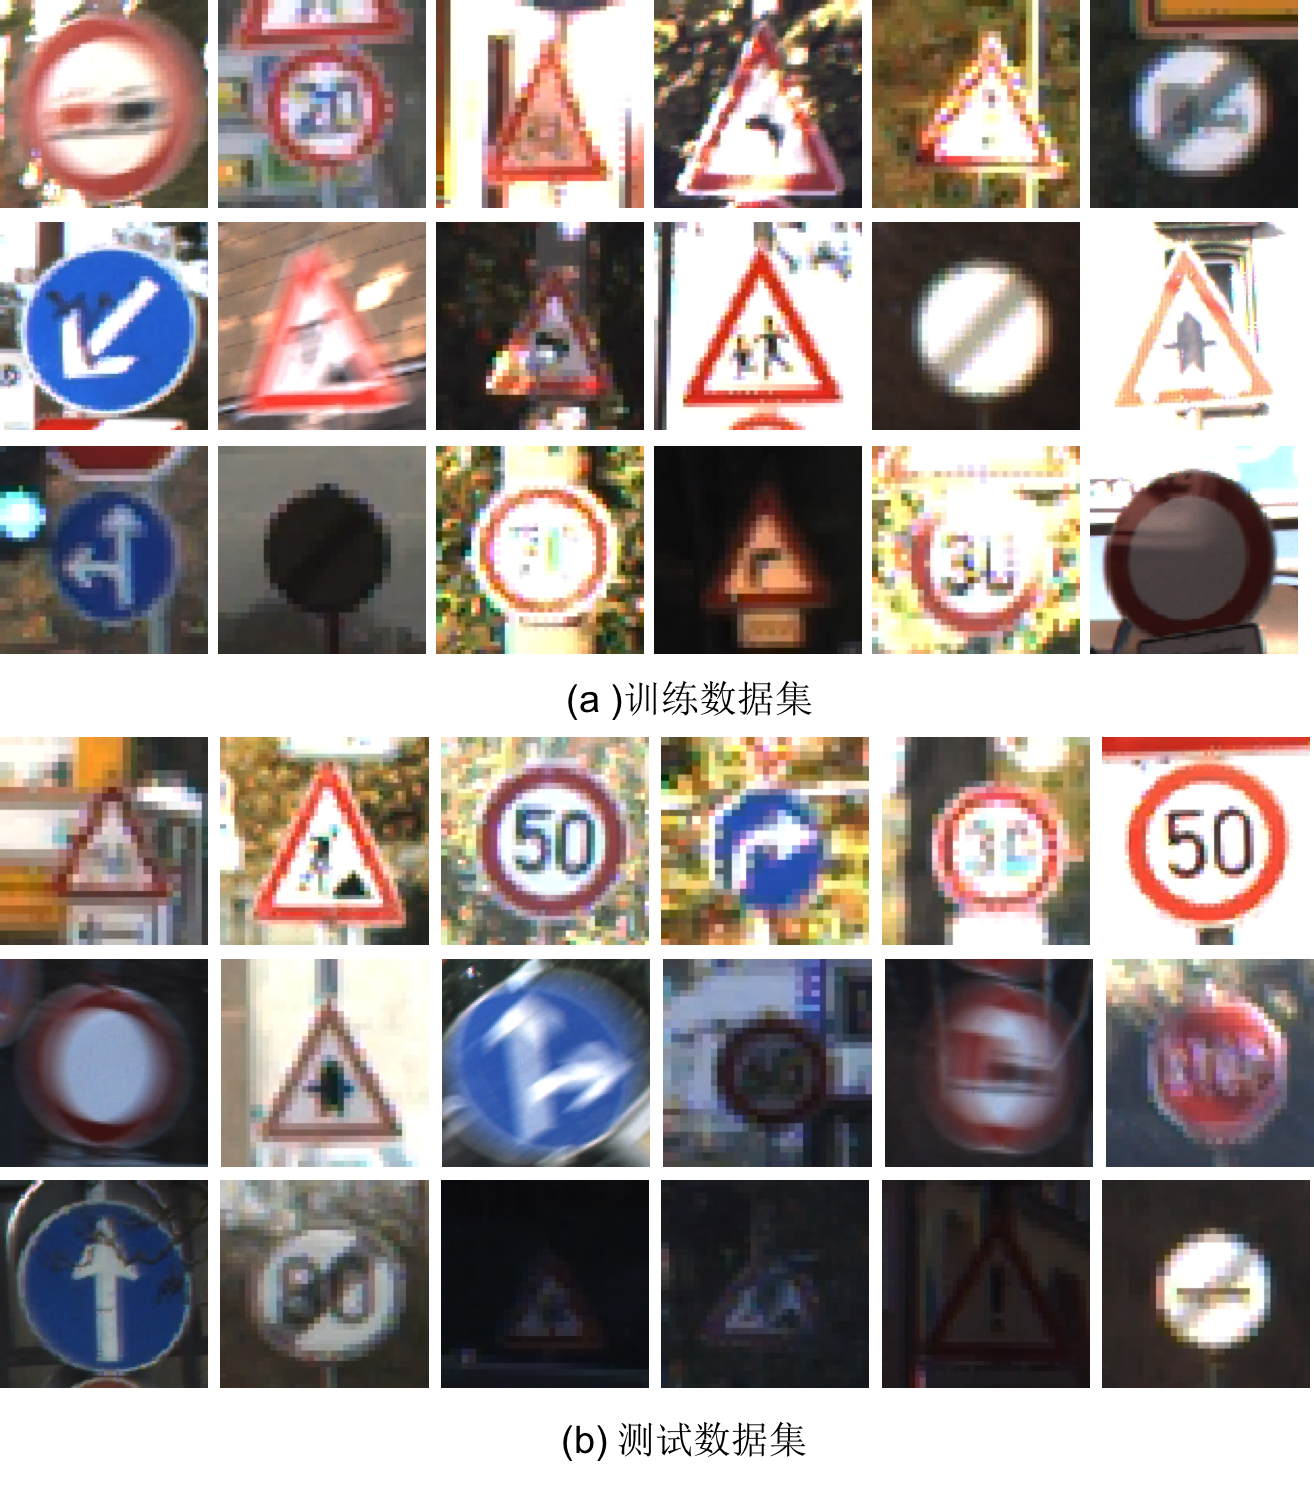
\includegraphics[width=0.9\linewidth]{tsr_train_test.png}
\caption{GTSRB图像样本。图中(a)是一些不同种类的训练交通标志样本,(b)是部分不同环境因素下测试交通标志样本。交通标志图像具有不同的视角、遮挡、模糊程度和尺寸变化。真实世界的环境因素也会对拍摄到的交通标志产生影响,在不同的车速、光照和天气条件下,采集到的图像会有很大的区别。此外,交通标志牌的褪色和磨损,不同时期布置的交通标志牌之间的差异等因素,都会给识别任务带来极大的困难与挑战。}
\label{fig:tsr_data}
\end{figure*}


本章我们以交通标志识别为应用背景,对论文第二、三、四章提出的方法进行了验证、对比与分析。第二章我们对卷积神经网络的卷积层进行改进,提出了一种组合卷积卷积结构:自适应卷积层(SAM),来简化复杂卷积神经网络的设计过程。SAM结构以Inception~\cite{szegedy2014going,szegedy2015rethinking,szegedy2016inception}为基础框架,结合了最大输出单元(Maxout)~\cite{goodfellow2013maxout},残差网络(ResNet)~\cite{he2015deep}和网络中的网络(NIN)~\cite{DBLP:journals/corr/LinCY13}四个模型的优势,可以有效地简化复杂深层网络的设计过程。第三章我们对卷积神经网络的池化层进行改进,提出了随机区域池化方法(SAP)来实现特征层的数据増广。SAP通过对池化区域进行随机的仿射变换,对特征进行重采样,在不影响特征空间样本分布的情况下对特征进行扰动,增加特征的多样性,最终实现特征増广,可以有效地提高网络的泛化能力。第四章我们提出了一种卷积神经网络模型压缩与加速方法,先通过主导卷积核分解对卷积层进行参数压缩与网络加速,再通过知识预回归的训练方法来尽量弥补压缩造成的精度损失。本章针对交通标志识别任务,对第二章和第三章的网络模型进行了测试与对比,并将两种方法进行结合,最后采用第四章的方法对模型进行加速,加快网络的推理速度,减少网络预测时间。本章其余内容组织如下:第~\ref{sec:seg:relate}节简要回顾了交通标志识别的相关研究工作;第\ref{sec:seg:model}节详细介绍了如何将组合卷积结构、随机区域池化和网络加速方法共同应用于交通标志识别任务;第~\ref{sec:seg:exp}节对实验结果进行了分析与讨论;第~\ref{sec:seg:conclusion}是对本章主要内容的总结。

\section{相关工作}
\label{sec:seg:relate}

交通标志的检测与识别是无人驾驶汽车和高级辅助驾驶技术中的一个重要研究课题。很多传统的机器学习方法致力于解决真实环境中由于尺寸、视角和清晰度的不同所产生的识别难题。2005年,Bahlmann等人~\cite{bahlmann2005system}综合考虑颜色、形状和运动信息,采用哈尔小波特征进行交通标志的检测、跟踪与识别。该方法具有较大的计算量,并且识别精度较低,虽然综合了交通标志颜色、形状和相机运动等信息,但是没有考虑到图像上下文的信息。2010年,Le等人~\cite{le2010real}采用支持向量机(SVM)对视频流中的颜色块进行检测,检索出交通标志可能出现的区域。Le等人重点研究了不同天气情况对交通标示识别的影响,但是该方法仅仅考虑了交通标志的颜色信息,且计算量较大。2011年,Zaklouta等人~\cite{zaklouta2011traffic}分别采用KD树和随机森林的方法对交通标志进行识别,论文还对比了不同尺度的HOG特征和距离变换函数对交通标志识别的影响。实验结果表明随机森林结合细粒度的HOG特征可以取得较好的识别率,但是Zaklouta等人并没有在论文中考虑交通标志的颜色信息。2012年,Lu等人~\cite{lu2012sparse}提出了一种基于稀疏编码的交通标志识别方法。2015年,Haloi等人~\cite{haloi2015novel}提出了一种基于概率潜在语义分析模型(Probabilistic Latent Semantic Analysis,pLSA)的交通标志识别系统,该系统采用由SIFT特征构成的词袋模型对图像的形状和交通标志的类别分别进行识别。Haloi等人的方法具有较快的识别速度,但是该方法也没有考虑交通标志的颜色和图像上下文信息。


基于卷积神经网络的识别方法在交通标志识别任务中取得了更好的识别率,2011年,Sermanet等人~\cite{sermanet2011traffic}在2011年的GTSRB交通标示识别竞赛中,采用具有两层结构的多尺度卷积神经网络逐层地学习特征,取得了98.97\%的识别率,超过了人类98.84\%~\cite{stallkamp2011german}的识别水平。之后,Sermanet等人进一步增加网络的参数规模,忽略图像的颜色信息,采用灰度图对网络进行训练和测试,在GTSRB数据集上取得了99.17\%的识别率。Sermanet等人采用的卷积网络只有两层的深度,没有充分挖掘出深层网络在特征提取方面的能力,两层网络所具有的感受野无法充分的提取图像的上下文信息。同年,Cirecsan等人~\cite{cirecsan2011committee}训练了25个具有三个卷积层和两个全连接层的卷积神经网络,并对输入图像进行了数据増广,采用多模型平均的方式,在GTSRB数据集上取得了99.46\%的识别率。该方法的主要缺点在于需要训练多个卷积神经网络模型,消耗大量的参数与计算量。2015年,Haloi~\cite{haloi2015traffic}等人结合空间变换网络~\cite{jaderberg2015spatial}和改进的Inception~\cite{szegedy2014going,szegedy2015rethinking,szegedy2016inception}结构,来提取具有平移、旋转和缩放不变性的特征,在GTSRB数据集上取得了99.81\%的识别率。该方法在GTSRB数据集上取得了最高的识别率,但是网络参数过多,计算量加大,很难应用于实际场景。2016年,Zhu等人~\cite{zhu2016traffic}联合腾讯地图发布了一个交通标示检测与识别的数据集清华-腾讯100K,该数据集图像主要来自腾讯街景地图。此外Zhu等人提出了一个端到端的交通标志检测与识别卷积神经网络模型,该网络可以同时解决检测与识别问题。

\section{交通标志识别}
\label{sec:seg:model}

第二章我们提出了卷积层的一种改进方法组合卷积结构,第三章我们提出了池化层的一种改进方法随机区域池化,第四章我们提出了一种基于主导卷积核和知识预回归的网络模型压缩与网络加速方法。这三章内容可以有效地组合,用于视觉物体的识别任务。组合卷积结构和随机区域池化可以提高网络的识别率,主导卷积核通过对卷积层进行低秩分解来减少网络的参数与计算量,再通过知识预回归的训练方式来弥补由于模型压缩所产生的精度损失。本小结中,我们首先结合组合卷积结构和随机区域池化层,提出了一个具有特征增广的自适应卷积网络模型(Self-adaptive Network with Feature Augmentation,FASNet)。此外,为了压缩模型的参数规模,加快网络的预测时间,我们采用主导卷积核分解对FASNet进行压缩与加速。


\begin{table}[h]
\caption{FASNet网络结构。}

\label{tab:fas}
\centering
\begin{tabular}{ccccccc}
 \toprule[1.5pt]
%{\heiti 类型} & {\heiti 感受野/步长} & {\heiti 输出特征维度} & {\heiti 分支1} & {\heiti 分支2} & {\heiti 选择器} & {\heiti 参数} \\
\multirow{2}{*}{\heiti 类型} & \multirow{2}{*}{\heiti 感受野/步长} & \multirow{2}{*}{\heiti 输出特征维度} & \multicolumn{3} {c}{SAM结构} &  \multirow{2}{*}{\heiti 参数} \\
\cline{4-6} &&&  {\heiti 分支1} & {\heiti 分支2} & {\heiti 选择器} \\
\midrule[1pt]
卷积层 & 3$\times$3/1 & 32$\times$32$\times$64 & - & - & - & 1.73 K \\
卷积层 & 3$\times$3/1 & 32$\times$32$\times$128 & - & - &  - & 73.73 K \\
\hline
SAP池化层 & 2$\times$2/2 & 16$\times$16$\times$128 & - & - & - & - \\
\hline
SAM卷积层 & - & 16$\times$16$\times$128 & 96 & 96  & 128 & 0.38 M \\
SAM卷积层 & - & 16$\times$16$\times$128 & 96 & 96 & 128 & 0.38 M \\
SAM卷积层 & - & 16$\times$16$\times$256 & 96 & 96 & 256 & 0.43 M \\
\hline
SAP池化层 & 2$\times$2/2 & 8$\times$8$\times$256 & - & - & - & - \\
\hline
SAM卷积层 & - & 8$\times$8$\times$256 & 160 & 160 & 256 & 1.27 M \\
SAM卷积层 & - & 8$\times$8$\times$256 & 160 & 160 & 256 & 1.27 M \\
SAM卷积层 & - & 8$\times$8$\times$512 & 160 & 160 & 512 & 1.43 M \\
\hline
全局池化 & 8$\times$8/8 & 1$\times$1$\times$512 & - & - & - & - \\
\hline
全连接层 & - & 43 & - & - & - & 22.02 K \\
\hline
softmax层 & - & 43 & - & - & - & -  \\
 \bottomrule[1.5pt]
\end{tabular}
\end{table}


自适应卷积模块(Self-Adaptive Module,SAM)的设计初衷是简化复杂卷积神经网络的设计过程。在SAM结构中,我们融合了多种有效的卷积网络结构,例如Inception~\cite{szegedy2014going,szegedy2015rethinking,szegedy2016inception},Maxout\cite{goodfellow2013maxout},ResNet~\cite{he2015deep}和NIN~\cite{DBLP:journals/corr/LinCY13}。SAM的结构如图~\ref{fig:sam}所示,以Inception为基础框架,我们在SAM结构中引入四条分支和一个选择器。其中两条简单分支分别具有不同的深度和感受野,一条最大化输出Maxout分支用于增强SAM的非线性特征逼近能力,一条残差分支用于加快模型的收敛速度。选择器除了可以用于特征的选择,减少特征维度,优化模型的计算量之外,同时可以增强局部感受野范围内特征的非线性。相比于传统的卷积层,SAM卷积层具有更自由的模型深度和感受野,更强的拟合能力和参数收敛速度。因此在FASNet网络结构中,我们大量采用SAM卷积层来替换掉传统的卷积层。根据卷积神经网络可视化方面的经验,卷积网络的前几层一般是在提取一些简单特征,因此对于FASNet的前两层,我们依然保留了传统的卷积层。

随机区域池化(Stochastic Area Pooling,SAP)的提出主要用于对特征层进行增广,即特征增广。在标注样本有限的情况下,数据增广是提高物体识别率的简单而有效的方法,从简单的平移和水平翻转的数据增广方式,到复杂的具有旋转、光照强度变化、像素值随机扰动的数据增广,都可以不同程度地提高测试数据的识别精度。众所周知,卷积神经网络的一个主要特点是分层的特征提取能力。而对于每层的特征图都具有与输入图像相似的结构与表示,因此我们提出了一种将数据增广扩展到隐层特征图的方法,即特征层数据增广,如图~\ref{fig:sap_sap}所示。随机区域池化由两步构成:基于随机仿射变换的池化区域选择和池化操作(如均值池化和最大池化)。在FASNet结构中,我们采用SAP池化层进行特征增广,来提高网络的泛化能力,提高网络的泛化能力。与第三章一致,本章我们同样采用最大池化作为FASNet网络中SAP层的后端的池化操作。

采用自适应卷积层与随机区域池化,FASNet的网络结构如表~\ref{tab:fas}所示,该网络由八个卷积层、三个池化层、一个全连接层和一个softmax层构成。其中八个卷积层中的前两个是传统的卷积层,具有 $3{\times}3$ 的感受野大小和 1 个像素的步长,用于提取图像的低级特征,其余六个为组合卷积结构,各分支与选择器的特征维度如表~\ref{tab:fas}所示;三个池化层中的前两个是随机区域池化,用于增加特征的多样性,提高网络的泛化能力,最后一个池化层为全局池化,用于生成固定大小的特征向量;全局池化之后的全连接层具有 43 个输出节点,分别代表了 43 类交通标志;网络最后的softmax层用于生成 43 类交通标志对应的概率分布。


\section{实验对比与分析}
\label{sec:seg:exp}

\subsection{实验设置}

基于开源深度学习框架caffe~\cite{jia2014caffe},我们设计并实现了交通标志识别网络FASNet,并在德国交通标志识别数据集GTSRB~\cite{stallkamp2012man}上,对FASNet进行了实验验证。所有的实验都是以数据并行的方式运行在具有两个GPU核心的单卡K80高性能服务器上。在所有对比实验过程中,我们均采用了批大小(Batch Size)为96的批量随机梯度下降法对FASNet进行训练。网络的初始学习率为 0.01,在训练过程中连续缩小 3 次,每次减小为原来的 $1/10$,直到学习率降低至 1e-5。整个训练过程中,我们采用了 0.9 的动量因子(Momentum)和 0.004 的权重衰减(Weight Decay)。对于随机区域池化层,我们采用与第三章相同的配置,即采用了均值为 0 标准差为 $5^{\circ}$ 的随机旋转,均值为 0 方差为 $1/4$ 输入特征尺寸的随机平移。数据预处理方式与前面三章略有不同,因为GTSRB训练图像的尺寸各不相同,因此我们无法像前三章那样计算各位置的像素均值,这里我们计算所有训练图片的BRG像素均值,用于对训练和测试图像去平均化处理。


\subsection{对比实验}

\begin{table}[h]
\centering
\caption{SAMNet,SAPNet,FASNet在GTSRB数据集上性能对比。}
\label{tab:3cmp}
\begin{tabular}{L{3cm}C{2cm}C{2cm}}
 \toprule[1.5pt]
{\heiti 模型} & {\heiti 参数规模} & {\heiti 识别率(\%)} \\
\midrule[1pt]
SAMNet & 3.34 M & {99.12} \\
SAPNet & 3.03 M & {99.50} \\
FASNet & 8.04 M & {99.66}\\
 \bottomrule[1.5pt]
\end{tabular}
\end{table}

德国交通标志识别数据集GTSRB一共具有 51,839 张图像,43 类交通标志,其中包括 39,209 张训练图像和 12,630 张测试图像。GTSRB中的图像具有不同的观测视角、不同程度的遮挡和不同的图像尺寸。在训练和测试的过程中,我们采用双线性差值将所有的图像转化为 $32{\times}32$ 像素大小的图像。在GTSRB数据集上,我们对第二章提出的SAMNet,第三章提出的SAPNet和本章提出了FASNet分别进行了实验测试与对比分析,实验结果如表~\ref{tab:3cmp}所示。SAMNet与SAPNet的对比可以看出,在网络参数规模相近的情况下,两个网络均取得了超过人类水平98.84\%的识别性能,尽管SAMNet具有更多的参数数量,但是识别率反而低于SAPNet。由此可见,组合卷积结构SAM对卷积层的优化确实是有效的,多分支加选择器的设计在简化网络的设计的同时,可以保证网络的识别能力。但是这种冗余的设计带来了额外的参数与计算开销。SAP对池化层的改进可以在基本不增加额外计算量的情况下,提高网络的泛化能力。两个方法的结合,即本章提出的FASNet,可以进一步提高测试样本的识别率。FASNet与其他方法的对比结果如表~\ref{tab:ocmp}所示。FASNet仅次于Haloi等人~\cite{haloi2015traffic}提出的Google Inception + Spatial Transformer Layer方法。

\begin{table}[h]
\centering
\caption{FASNet在GTSRB数据集上与其他方法的对比结果。}
\label{tab:ocmp}
\begin{tabular}{cc}
 \toprule[1.5pt]
{\heiti 模型} &  {\heiti 识别率(\%)} \\
\midrule[1pt]
Random Forest~\cite{zaklouta2011traffic} & 96.14 \\
pLSA~\cite{haloi2015novel} & 98.14 \\
Human Performance~\cite{stallkamp2011german} & 98.84 \\
Multi-Scale CNN~\cite{sermanet2011traffic} & 98.87 \\
Committe of CNNs~\cite{cirecsan2011committee} & 99.46 \\
Google Inception~\cite{jaderberg2015spatial} & 99.57 \\
Google Inception + Spatial Transformer Layer~\cite{haloi2015traffic} & 99.81 \\
\hline
FASNet &  {99.66} \\
 \bottomrule[1.5pt]
\end{tabular}
\end{table}

\subsection{模型压缩与加速}
\label{app:acc}

\begin{figure*}[t]
\centering
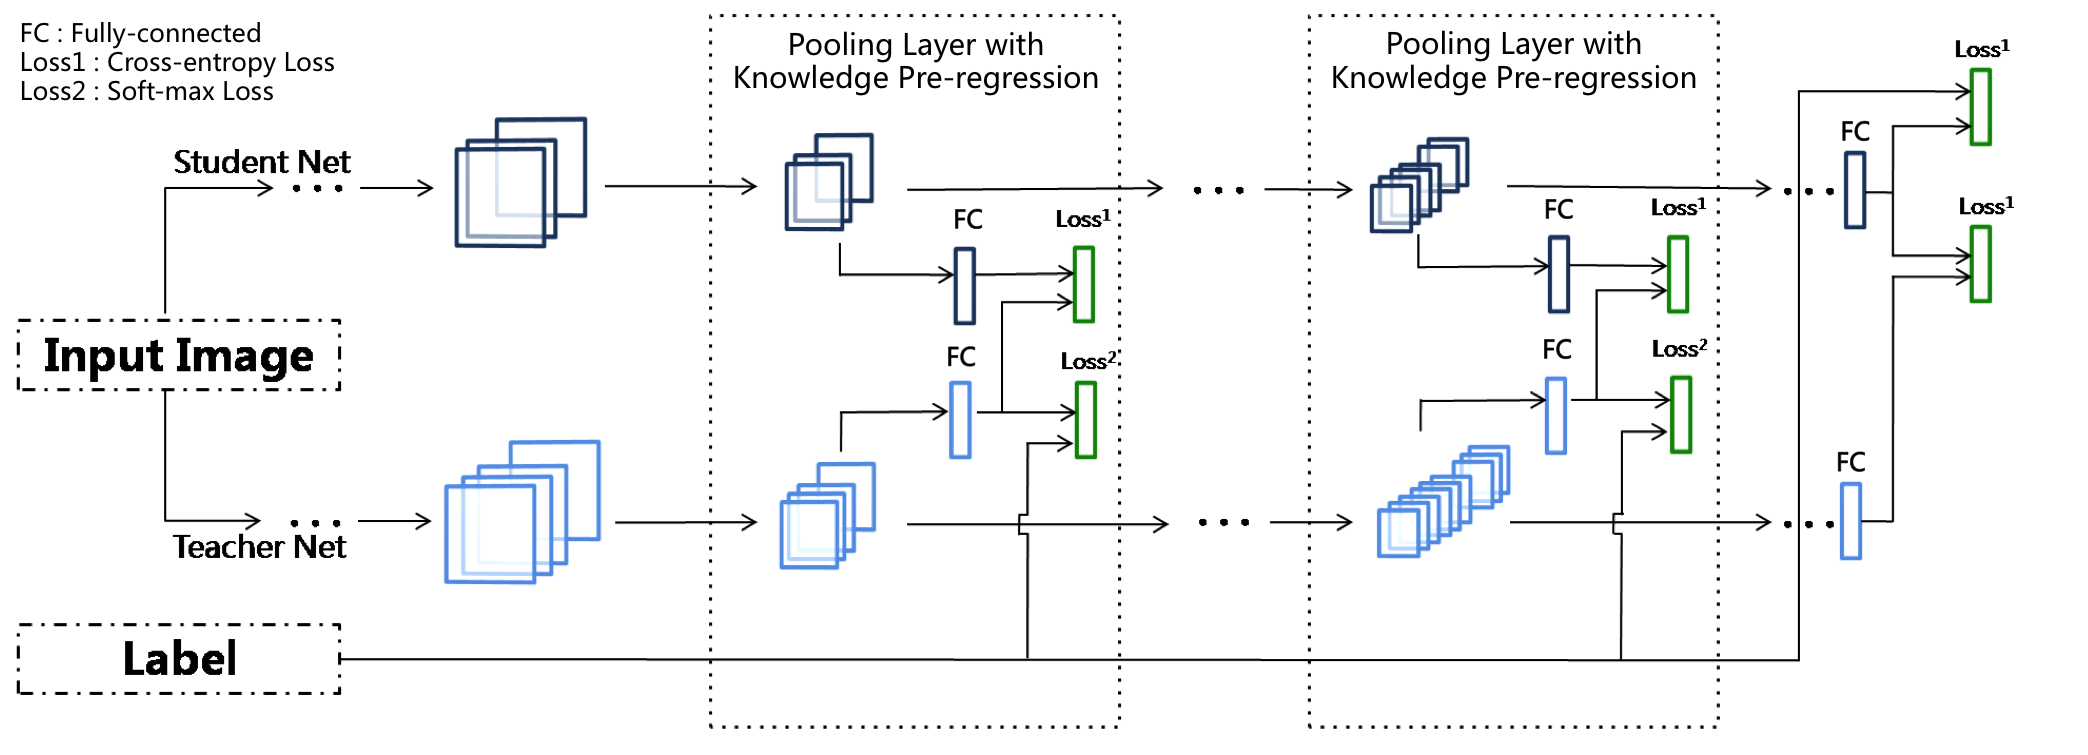
\includegraphics[width=1.0\linewidth]{acc_kp.png}
\caption{FastNet训练过程}
\label{fig:train}
\end{figure*}

FASNet网络具有 5.23M 参数数量和 636.70M 的浮点乘加运算,如表~\ref{tab:fast}所示。FASNet的参数规模和计算量较大,很难对其进行部署应用。因此我们采用1比1的主导卷积核分解对FASNet中的卷积层进行参数压缩,得到一个参数和运算规模较小,推断速度更快的网络结构FastNet。FastNet与FASNet的网络结构、参数和运算规模的对比如表~\ref{tab:fast}所示。压缩后的FastNet仅仅具有 0.37M 的参数数量,是FASNet的 7.07\%。在浮点乘加运算上,FastNet是FASNet的 7.17\%,因此FastNet的推断速度会比FASNet快10倍以上。

\begin{table}[h]
\caption{FASNet与FastNet参数与运算规模对比。}
\label{tab:fast}
\centering
\begin{tabular}{ccc|ccc}
\hline
\multicolumn{3}{c|}{\heiti FASNet} & \multicolumn{3}{c}{\heiti FastNet(1比1)} \\
\cline{1-3}
\cline{4-6}
{\heiti 结构} & {\heiti 参数} & {\heiti 浮点运算} & {\heiti 结构} & {\heiti 参数} & {\heiti 浮点运算} \\
\midrule[1pt]
卷积层 & 1.73 K & 1.77 M & 卷积层  & 1.73 K & 1.77 M\\
卷积层 & 73.73 K & 75.50 M & DK卷积层 & 8.77 K & 8.98 M\\
\hline
SAP池化层  & - & - & SAP池化层  & - & - \\
\hline
SAM卷积层 & 0.38 M & 97.52 M & DK卷积层 & 17.54 K & 4.49 M \\
SAM卷积层 & 0.38 M & 97.52 M & DK卷积层 & 17.54 K & 4.49 M\\
SAM卷积层 & 0.43 M & 110.10 M & DK卷积层 & 33.92 K & 8.68 M\\
\hline
SAP池化层  & - & - & SAP池化层  & - & - \\
\hline
SAM卷积层 & 1.27 M & 81.26 M & DK卷积层 & 67.84 K & 4.34 M \\
SAM卷积层 & 1.27 M & 81.26 M & DK卷积层 & 67.84 K & 4.34 M \\
SAM卷积层 & 1.43 M & 91.75 & DK卷积层 & 0.13 M & 8.54 M\\
\hline
全局池化  & - & - & SAP池化层  & - & - \\
\hline
全连接层 & 22.02 K & 22.02 K & 全连接层 & 22.02 K & 22.02 K \\
\hline
softmax层 & - & - & SAP池化层  & - & - \\
\midrule[1pt]
合计 & 5.23 M & 636.70 M & 合计  & 0.37 M & 45.65 M \\
 \bottomrule[1.5pt]
\end{tabular}
\end{table}

采用第四章中知识预回归的训练方法对FastNet进行训练,以FASNet为学习对象,即教师网络,我们对FastNet进行训练,训练过程如图~\ref{fig:train}所示。我们对FASNet和FastNet的3个池化层分别进行预回归训练,在训练过程中,对于教师网络FASNet,我们采用最大池化代替了原网络中的随机区域池化,让FASNet在逐层监督的过程中可以产生相对稳定不变的监督信息,更为有效地指导学生网络FastNet的学习,加快FastNet网络的收敛速度。通过预回归训练,FastNet的取得了99.27\%的识别率。

\begin{figure}[h]
  \centering%
  \begin{subfigure}{0.45\textwidth}
    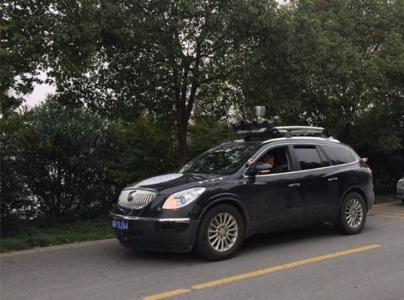
\includegraphics[width=1\linewidth]{tsr_car2.png}
    \caption{THU-IV2。}
  \end{subfigure}%
  \hspace{1em}%
  \begin{subfigure}{0.4\textwidth}
    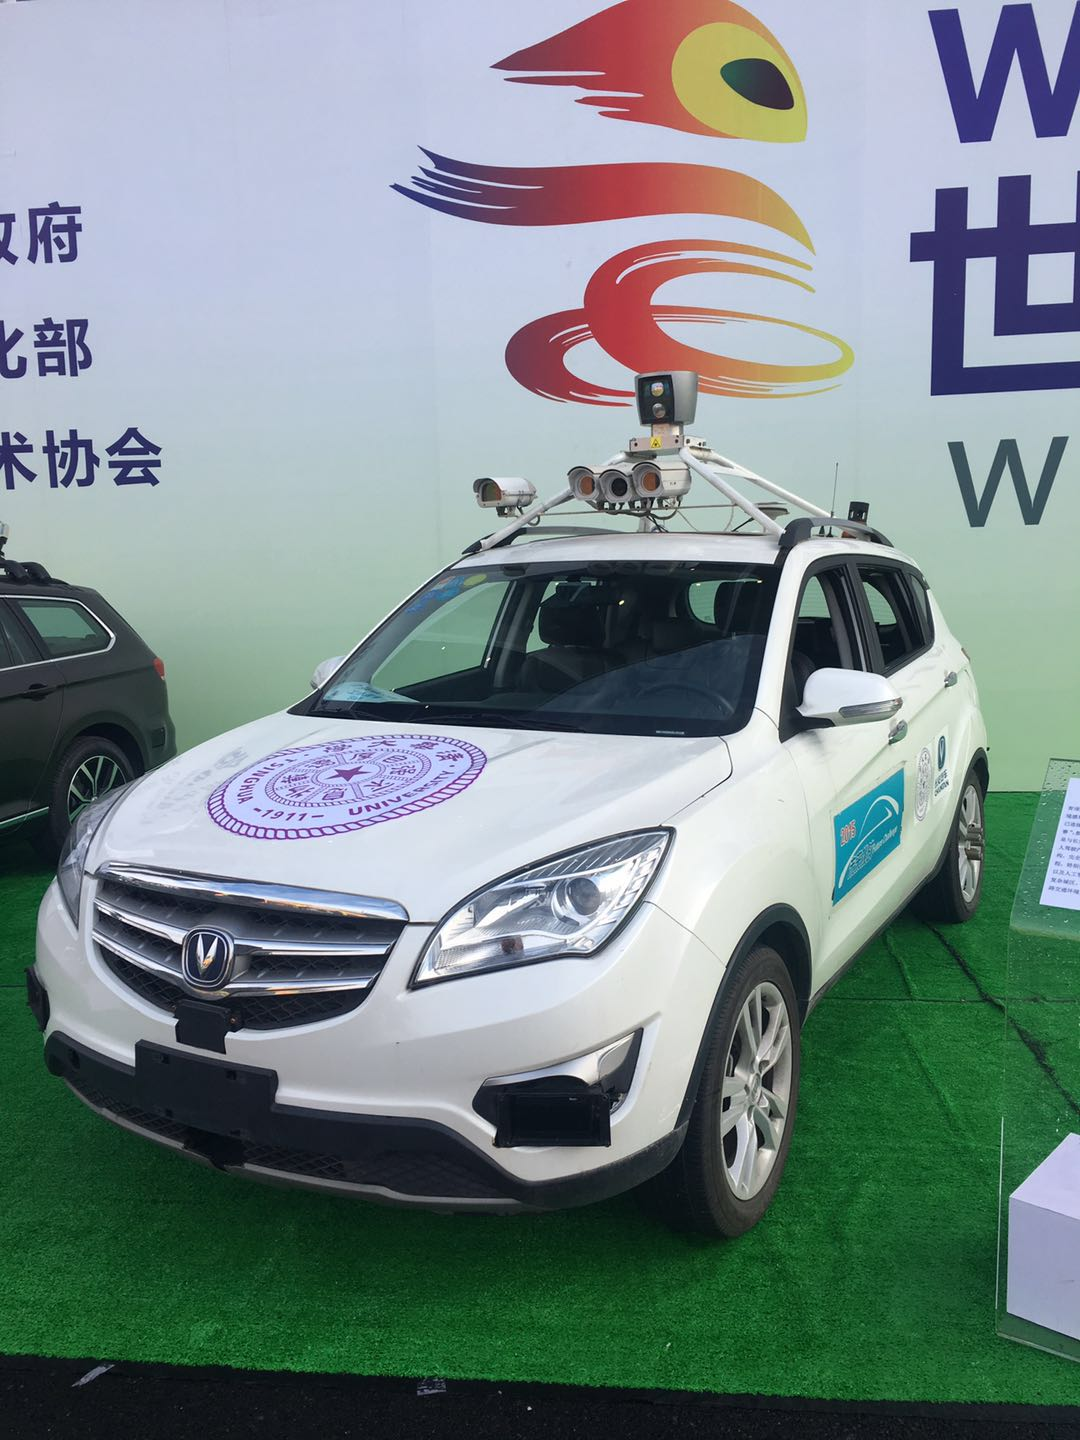
\includegraphics[width=1\linewidth]{tsr_car3.jpg}
    \caption{THU-IV3。}
  \end{subfigure}
  \caption{THU-IV2 和 THU-IV3 第二代与第三代无人驾驶汽车。}
  \label{fig:tsr_car}
\end{figure}

\subsection{无人驾驶汽车上的交通标志检测与识别}

上文中,我们已经成功地实现了基于卷积神经网络的交通标志识别与模型压缩与加速。本小结将讨论在无人驾驶汽车上,交通标志的检测与识别问题。在国家自然科学基金委所支持的重大研究项目”视听觉信息的认知计算“中,我所在的课题组自主研发了 THU-IV1、THU-IV2 和 THU-IV3 三款无人驾驶汽车,其中 THU-IV2 和 THU-IV3 第二代与第三代无人驾驶汽车如图~\ref{fig:tsr_car}所示。基于第三代实验平台 THU-IV3,我们开发了交通标志检测与识别系统。

\begin{figure}[b]
\centering
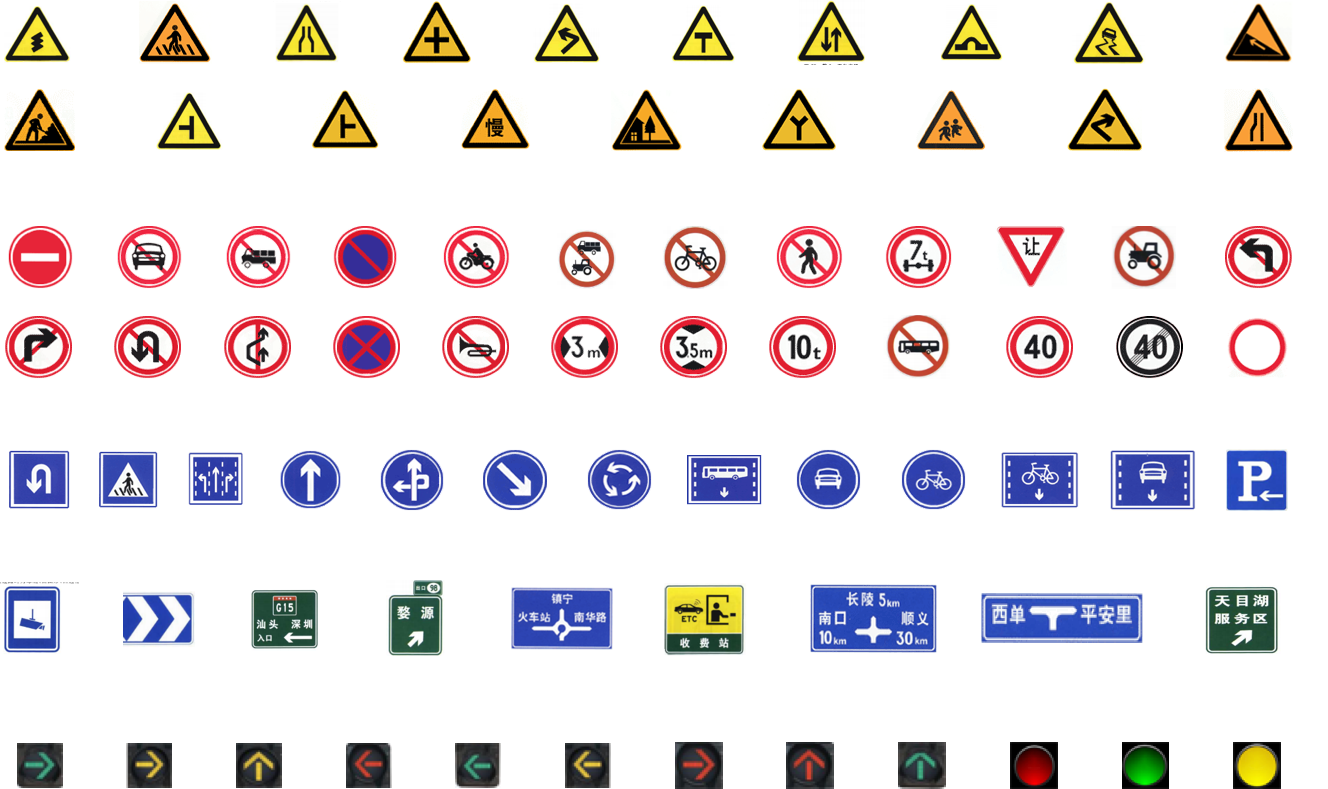
\includegraphics[width=1\linewidth]{tsr_types.png}
\caption{警告标志20类,禁令标志24类,指示标志13类,指路标志9类,交通灯12类。}
\label{fig:tsr_types}
\end{figure}

本章采用场景标注的方式来分割出原始图像中交通标志的位置,来实现交通标志检测的目的。场景标注旨在为输入图像的每一个像素都确定一个语义类别标签,本章采用卷积神经网络对不同位置的图像块进行语义分割,通过语义分割的结果来定位交通标志出现的具体位置。我们采集了2695张具有 $1280\times1024$ 像素大小的离线图像数据集,将其平均分为5份,采用交叉验证的方式,其中四份作为训练集,一份作为测试集。参考 GB5768-2009《道路交通标志和标线》国标中对于交通标志的定位,将交通标志和交通信号灯统一定义为78类,其中包括警告标志20类,禁令标志24类,指示标志13类,指路标志9类,交通灯12类,如图~\ref{fig:tsr_types}。


我们采用如图~\ref{fig:tsr_det2}、图~\ref{fig:tsr_det1}等检测结果类似的图像标注方法,左图对应于原始的输入图像,对于标注图像,我们采用矩形边界框,即形式如(左下角宽度坐标,左下角长度坐标,宽度,长度)的矩形边界框对交通标志进行标注,对于78类不同的交通标志,用1-78这78个整数来填充矩形边界框区域,图像的背景设置为0。尽管矩形边界框的标志方式相对于图像分割任务较为粗略,但是对于本章交通标志识别任务,这样的标志已经完全足够使用。

\begin{figure}
\centering
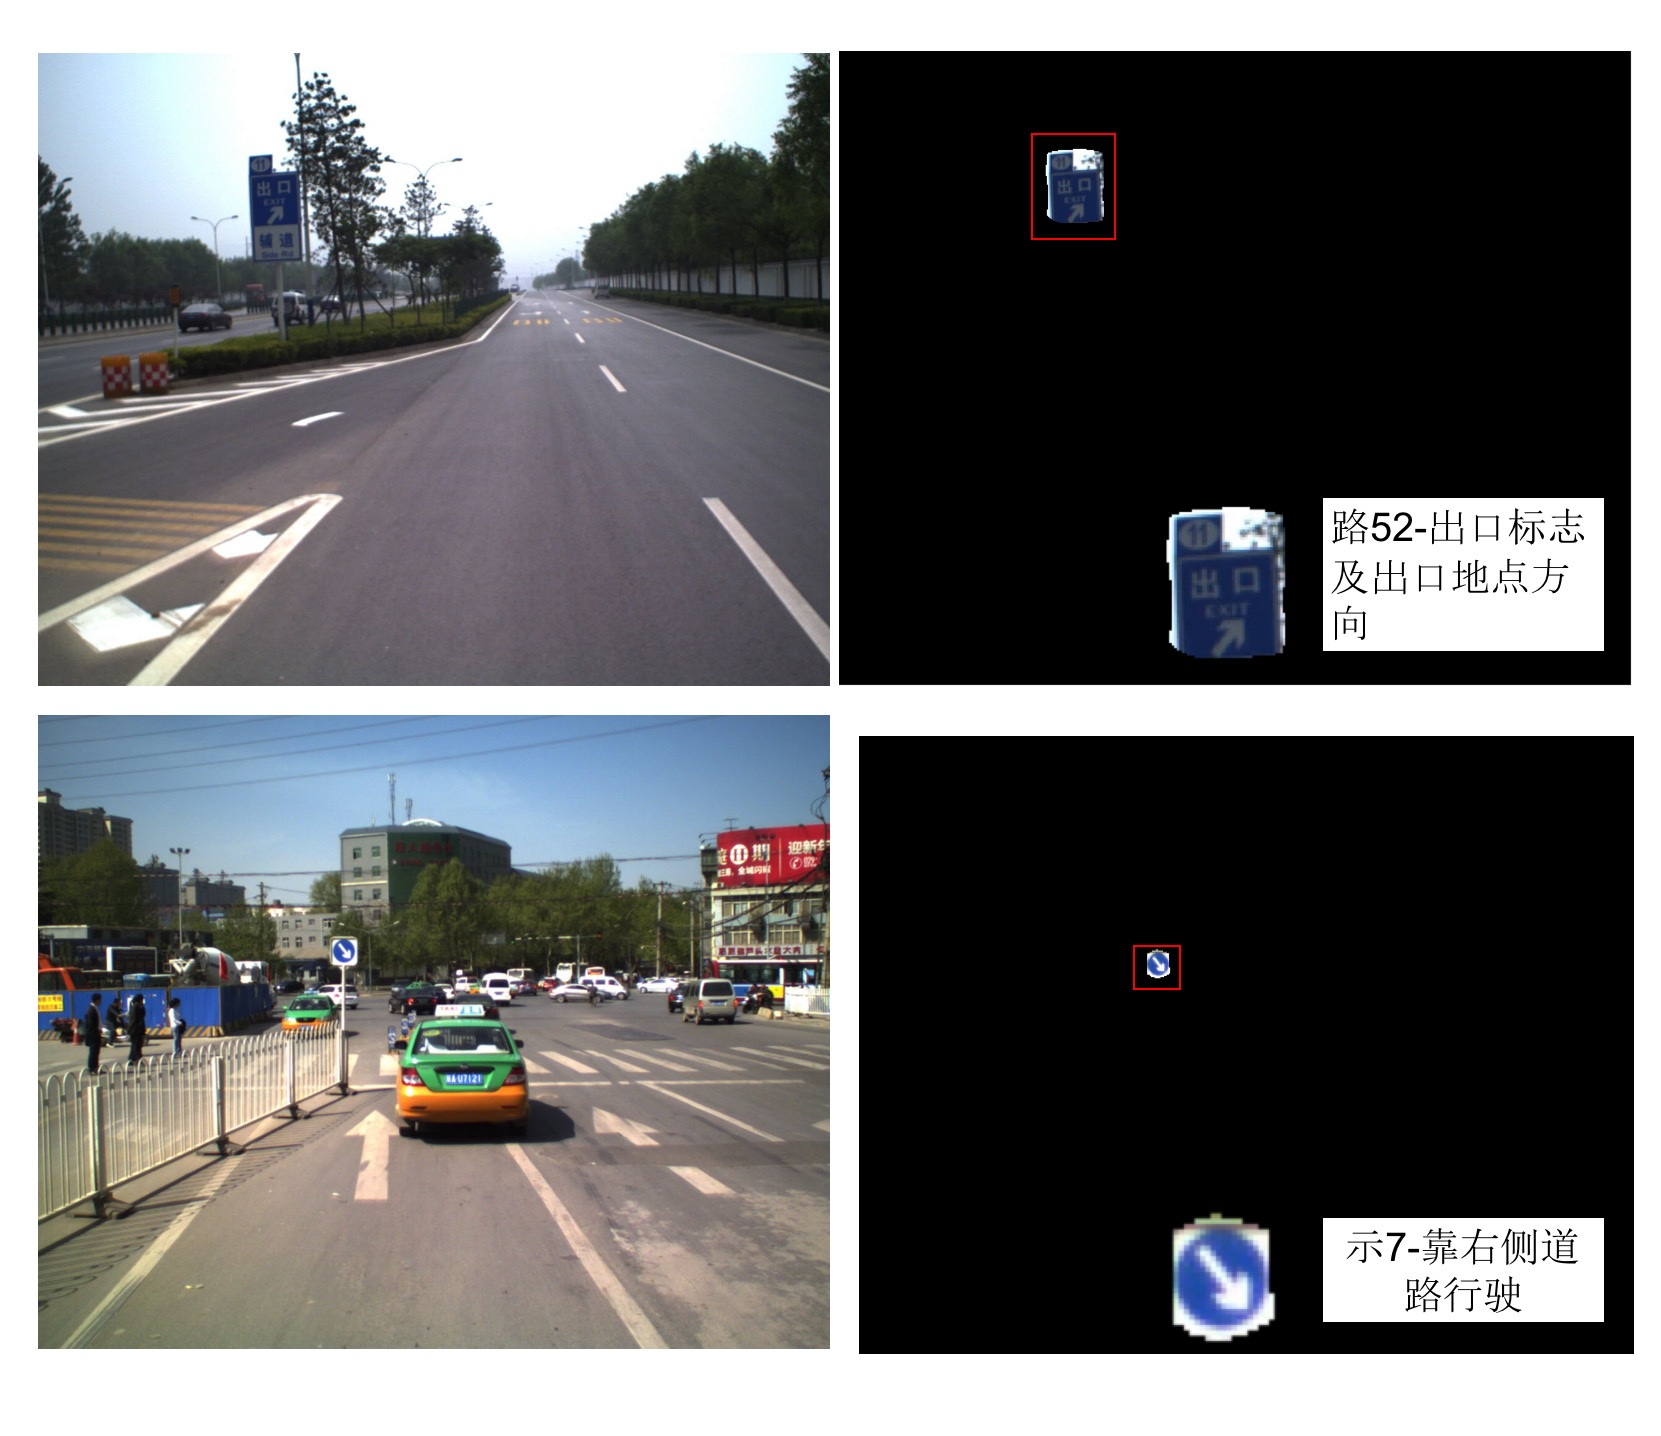
\includegraphics[width=1.0\linewidth]{tsr_det2.jpg}
\caption{指路标志与指示标志分割识别结果。}
\label{fig:tsr_det2}
\end{figure}

\begin{figure}
\centering
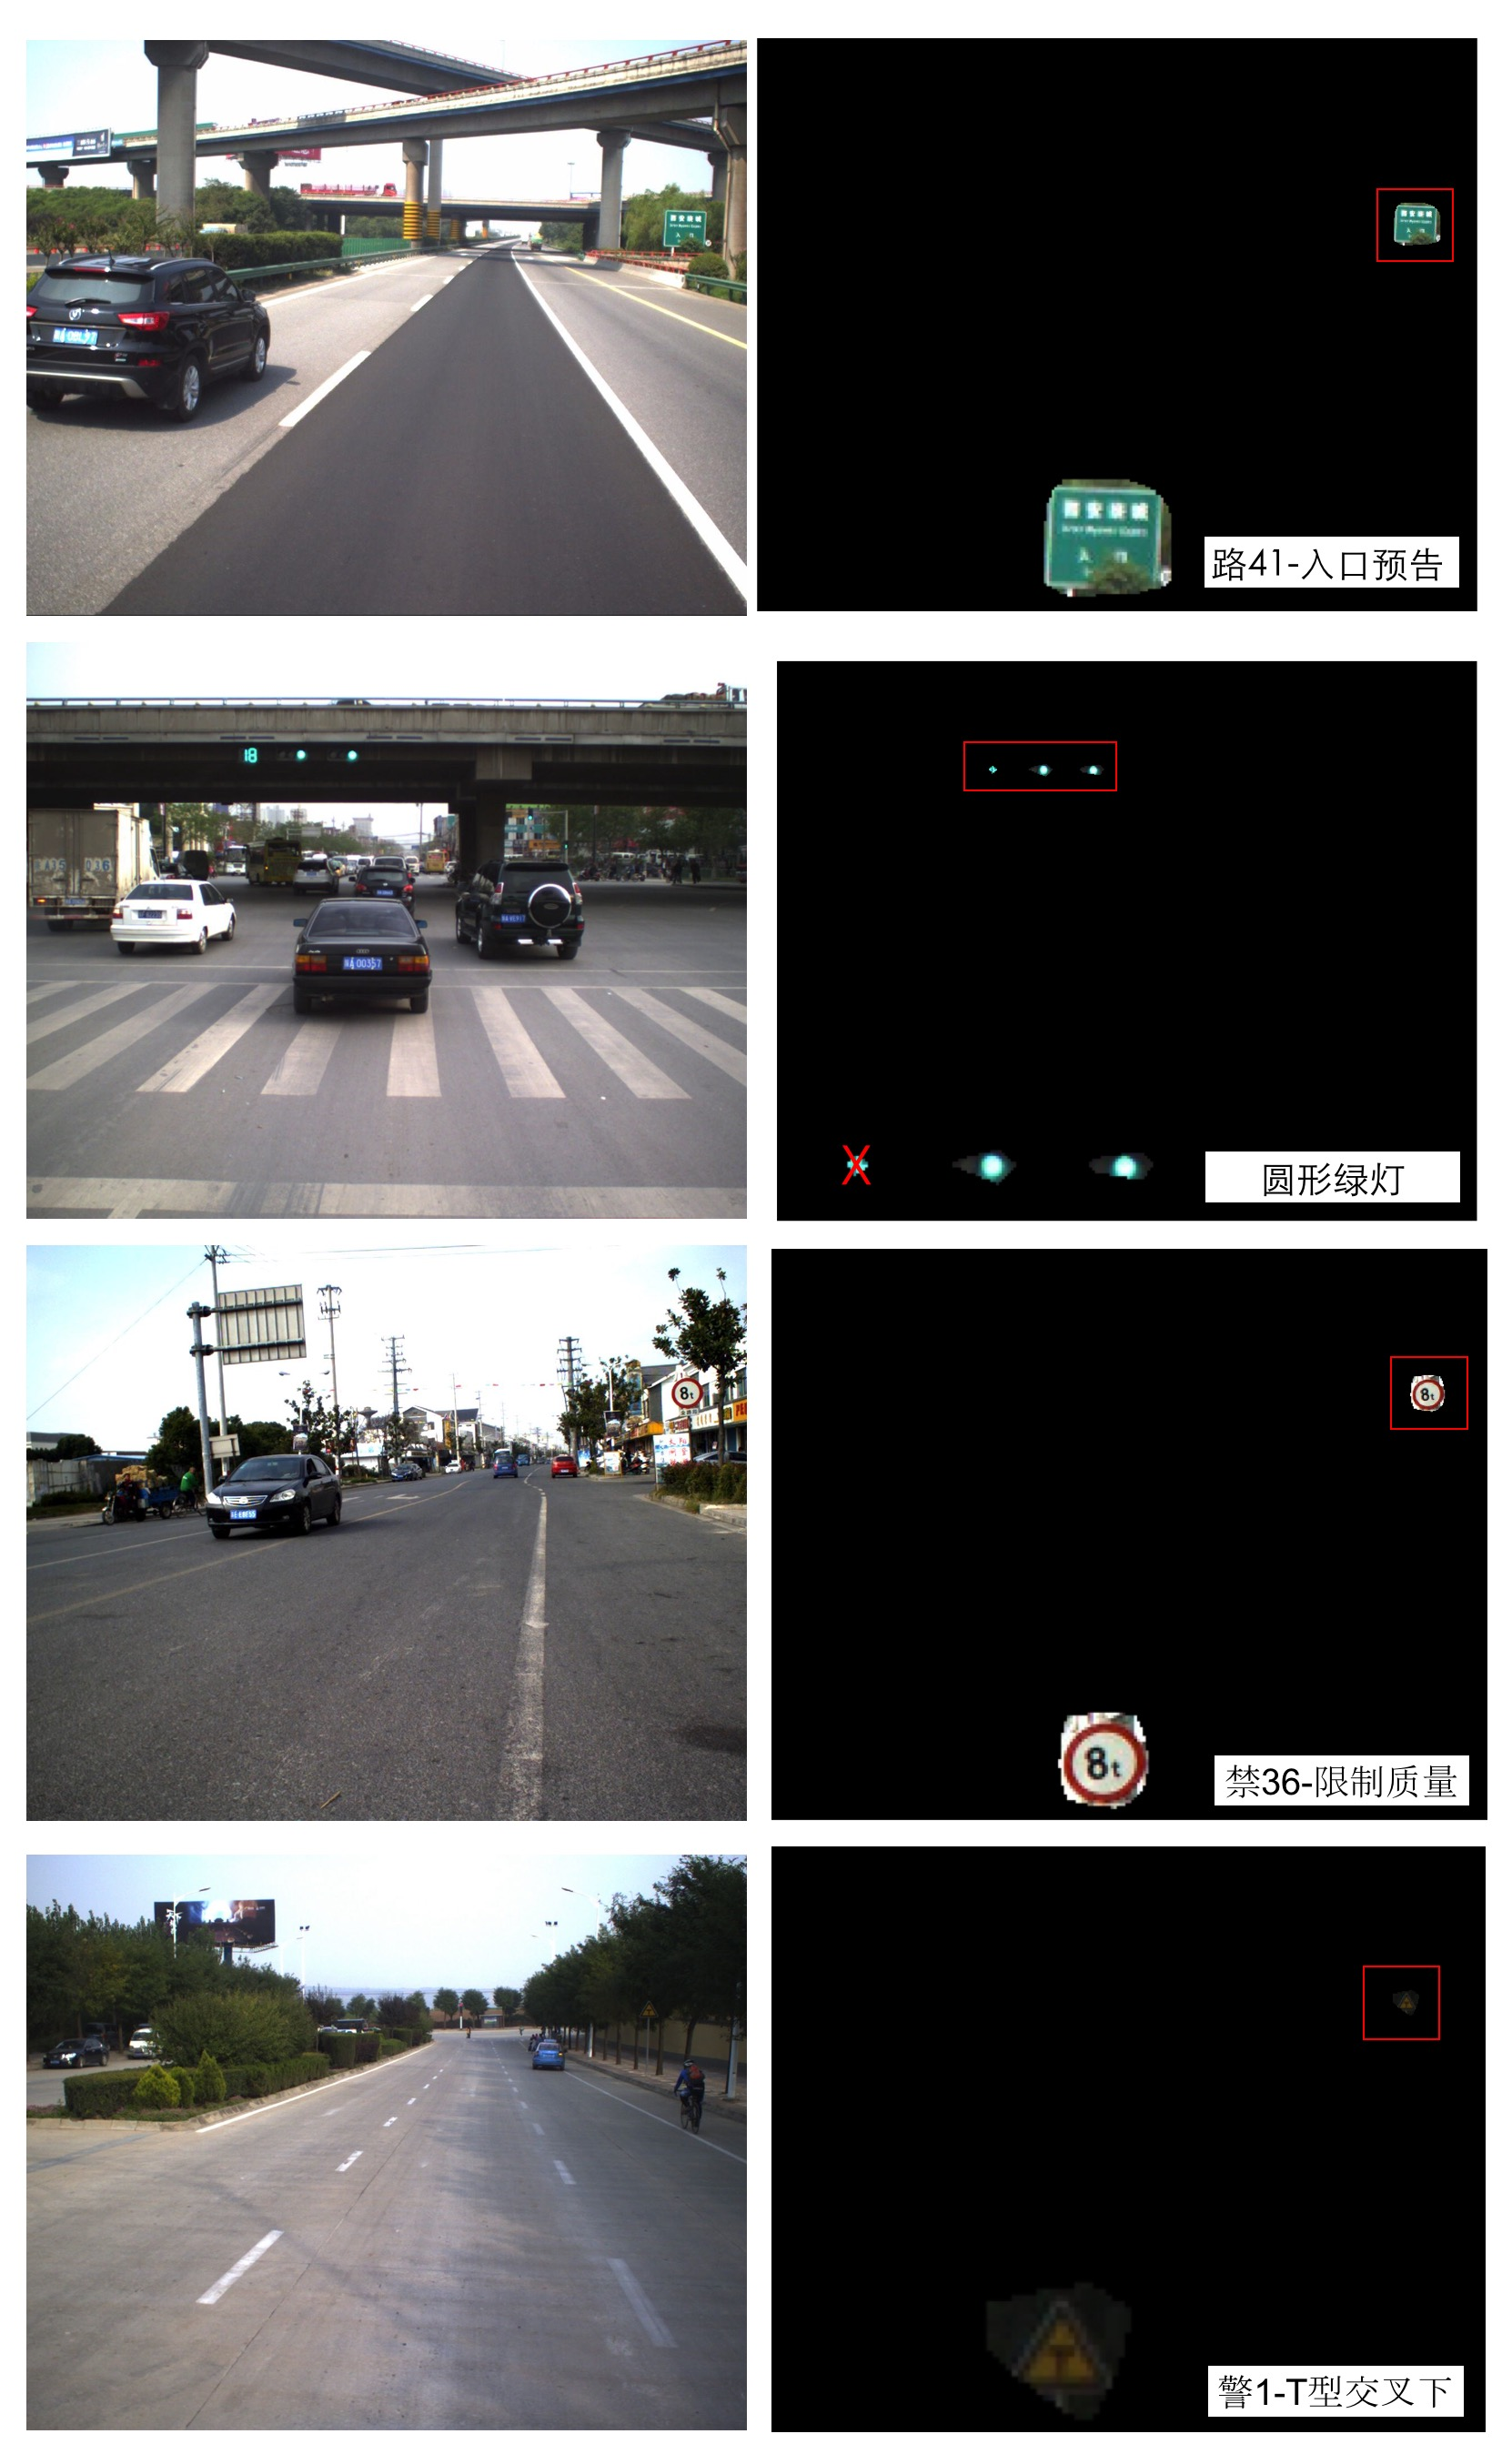
\includegraphics[width=1.0\linewidth]{tsr_det1.jpg}
\caption{指路标志、交通灯、禁令标志、警告标示分割识别结果。}
\label{fig:tsr_det1}
\end{figure}



我们采用上文提出的FASNet卷积神经网络模型进行图像的场景分割,采用全卷积~\cite{long2014fully}的方式进行图像分割,但是与~\cite{long2014fully}不同,我们采用双线性差值的方式对特征图进行上采样,还原成与原始输入图像相同的尺度大小,最后采用Softmax进行逐像素的回归分类。为了提高语义分割网络的性能和训练速度,我们采用第~\ref{app:acc}节在GTSRB数据集上预训练的模型参数对分割网络进行初始化,采用较小的学习率对分割网络进行参数微调。值得注意的是,对于GTSRB交通标志识别任务,仅仅具有43类,需要将其扩展为79类(78个交通标志类别和图像背景)。

在离线测试数据集上,网络的分割结果如图~\ref{fig:tsr_det2}和图~\ref{fig:tsr_det1}所示,图中分别列举了指路标志、交通灯、禁令标志、警告标示和指示标志等交通标志分割结果,对于前景与背景区分度较大的交通标志,分割算法均能取得较好的分割结果。但是对于图~\ref{fig:tsr_det1}中“警1-T型交叉下”交通标志,由于其前景与背景区分度较低,因此分割的边界较为粗略,但分割区域内也包含了完成的交通标志,对于无人驾驶汽车来说已经足够使用。图~\ref{fig:tsr_det1}是圆形交通信号灯的分割,测试结果给出了三个分割结果,但是最左侧的分割结果有误,未能成功的判断出该位置的标示的为红绿灯的剩余时间,而非圆形绿灯。

\section{本章小结}
\label{sec:seg:conclusion}

本章内容是前三章方法的一个综合应用,我们以交通标志识别为应用背景,对组合卷积结构和随机区域池化分别进行了实验验证。组合卷积结构可以有效地提高卷积层的识别能力和网络收敛速度,但是多条特征提取分支加选择器的冗余设计引入了更多的参数和计算量。随机区域池化方法可以在卷积网络的池化层进行特征増广,在基本不引入额外参数与计算量的情况下提高网络的泛化能力。组合卷积结构和随机区域池化作为通用的卷积和池化模块,可以有效地和其他网络结构配合使用。本章我们采用这两种方法构造了FASNet,在德国交通标志识别数据集GTSRB上取得了99.66\%的识别率。针对FASNet网络的参数与计算量较高问题,我们采用第四章中提出的主导卷积核分解方法对网络进行压缩,提出了FastNet结构,并采用知识预回归的训练方法对FastNet进行训练,最终实现了99.27\%的识别率。相对于原始的FASNet网络模型,FastNet具有近10倍的参数压缩比率和预测速度提升。最后,基于 THU-IV3 实验平台,我们进行了交通标志与信号灯的检测与识别实验。










